\documentclass[12pt, a4paper]{article}

\renewcommand{\baselinestretch}{1.5}
\pagenumbering{arabic}
\pagestyle{plain}

\usepackage[margin=2cm]{geometry}
\usepackage{polski}
\usepackage[utf8]{inputenc}
\usepackage{indentfirst}
\usepackage[fleqn]{amsmath}
\usepackage{graphicx}
\usepackage{float}
\usepackage[tableposition=top]{caption}
\usepackage{hyperref}
\graphicspath{ {../figures/}}
\hypersetup{
    colorlinks=true,
    linkcolor=blue,
    filecolor=magenta,      
    urlcolor=blue,
    pdfpagemode=FullScreen,
    }

\author{Jakub Bożek}

\title{Sprawozdanie z HCA}
\begin{document}

\begin{titlepage}
    \centering
    {\LARGE \bfseries Sprawozdanie z HCA \par}
    \vspace{1cm}
    
    {\Large Techniki eksploracji danych wielowymiarowych \par}
    \vspace{2cm}
    
    {\LARGE \bfseries Jakub Bożek \par}
    \vspace{0.5cm}
    
    {\large 285665 \par}
    \vspace{0.5cm}
    
    {\large Bioinformatyka, II rok \par}
    \vspace{2cm}
    
    {\Large \today \par}
    
    \newpage
    \thispagestyle{empty}

    \tableofcontents
\end{titlepage}

\section{Wprowadzenie}

    \subsection{Opis problemu}
        Analiza podobieństwa związków chemicznych dla małej ilości informacji jest relatywnie prosta.
        Problem zaczyna się w momencie posiadania dużej ilości danych, tak jak w naszym przypadku.

    \subsection{Cel analizy}
        Znalezienie podobieństw pomiędzy wybranymi 20 pestycydami i ich uszeregowanie w mniejsze, łatwiejsze do interpretacji grupy.

    \subsection{Hipoteza badawcza}
        Wybrane związki będą wykazywały podobieństwo między sobą tworząc tzw. klastry, inaczej zbiory zawierające
        elementy podobne.

    \subsection{Oprogramowanie}
        Wszystkie elementy sprawozdania zostały stworzone przy pomocy języka programowania \href{https://docs.python.org/3.10/}{Python 3.10.12} z pomocą bibliotek:\\
        \href{https://numpy.org/doc/1.26/}{Numpy 1.26.2}\\
        \href{https://matplotlib.org/3.8.2/index.html}{Matplotlib 3.8.2}\\
        \href{https://pandas.pydata.org/pandas-docs/version/2.1.3/}{Pandas 2.1.3}\\
        \href{https://docs.scipy.org/doc/scipy-1.12.0/}{Scipy 1.12.0}\\
        \href{https://www.rdkit.org/docs/index.html}{Rdkit 2023.09.5}
        \label{link:Rdkit}



\section{Opis zbioru danych}

    Dla podanych nazw związków znalezione zostały ich kody Smiles, który jest 
    uniwersalnym przedstawieniem danej molekuły za pomocą, w uproszczeniu, ułożonych szeregowo pierwiastków.
    
    Następnie z pomocą biblioteki Rdkit$^{\ref{link:Rdkit}}$ znaleźliśmy deskryptory, które są liczbowym opisem molekuły.
    
    Tabela z zestawionymi deskryptorami posiada wymiar 20 x 210(liczba zmiennych x liczba obserwacji). Dane są w większości danymi
    zmiennoprzecinkowymi(float) lub całkowitymi(int).

\section{Metoda analizy}

    W celu zredukowania wymiaru naszych danych usunęliśmy obserwacje o zerowym wkładzie.
    Jeżeli kolumna wartości posiada wariancję równą 0 to znaczy, że wszystkie wartości są takie same.
    Po tej operacji nasza tabela skurczyła się do rozmiarów 20 x 147.
    
    Oprócz tego możnaby wykonać usunięcie wszystkich wierszy oraz kolumn w których występują puste pola, które
    uniemożliwiłyby nam dalszą analizę. W tym przypadku nie było to konieczne ze względu na brak ich występowania.

    Następnie przeprowadziliśmy autoskalowanie danych, co określane się wzorem:
    \begin{equation}
        z_{ij} = \frac{x_{ij} - \mu_j}{\sigma_j}
    \end{equation}
    gdzie:
    \begin{align*}
        z_{ij} &= \text{zmienna ustandaryzowana}\\
        x_{ij} &= \text{zmienna niestandaryzowana}\\
        \mu_j &= \text{średnia dla obserwacji}\\
        \sigma_j &= \text{odchylenie standardowae dla obserwacji}
    \end{align*}

    W wyniku autoskalowania, inaczej standaryzacji, zmienna uzyskuje wartość oczekiwaną 0 oraz odchylenie standardowe 1.

    Dla tak przetransformowanych danych przeprowadziliśmy HCA metodą pojedynczego wiązania(najbliższego sąsiada)
    oraz całkowitego wiązania(najdalszego sąsiada).
    W celu dogłębnejszej analizy dla każdej metody wiązania wybieramy po 2 metryki odległości, Euklidesową oraz Manhattan
    \begin{equation}
        d_{Euk}(x,y) = \sqrt{\sum_i (x_i - y_i)^2}\\
        d_{Manh}(x,y) = \sum_i |x_i - y_i|
    \end{equation}
    Oprócz tego, dodatkowo, przeprowadziliśmy HCA dla danych przed autoskalowaniem. Ja wybrałem metodę pojedynczego wiązania oraz metrykę odległości Euklidesowej.

\section{Wyniki analizy}

    \begin{figure}[H]
        \centering
        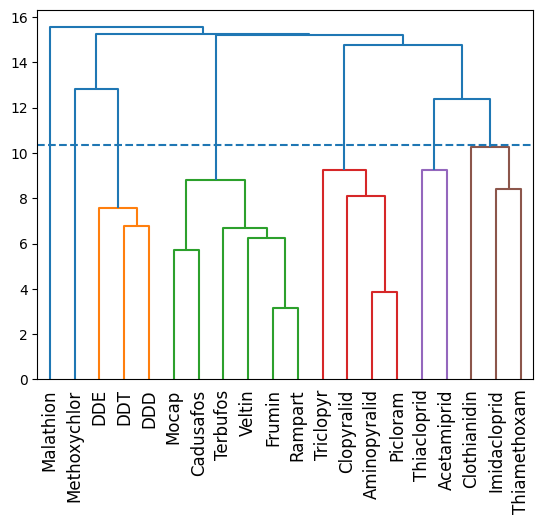
\includegraphics{wp_Euk.png}
        \caption{Dendrogram dla wiązania pojedynczego, metryka odległości Euklidesowej, dane autoskalowane}
    \end{figure}

    \begin{figure}[H]
        \centering
        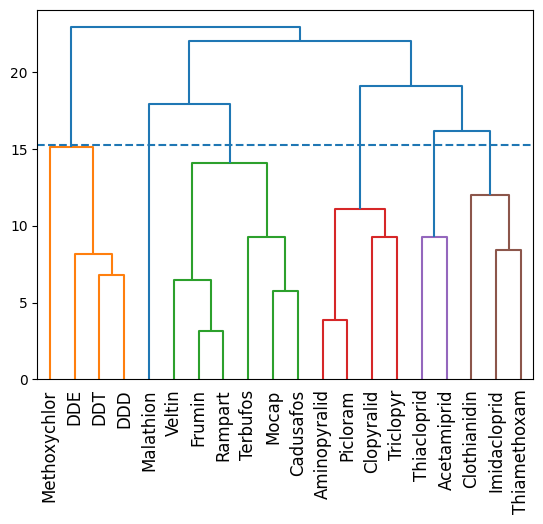
\includegraphics{wc_Euk.png}
        \caption{Dendrogram dla wiązania całkowitego, metryka odległości Euklidesowej, dane autoskalowane}
    \end{figure}

    \begin{figure}[H]
        \centering
        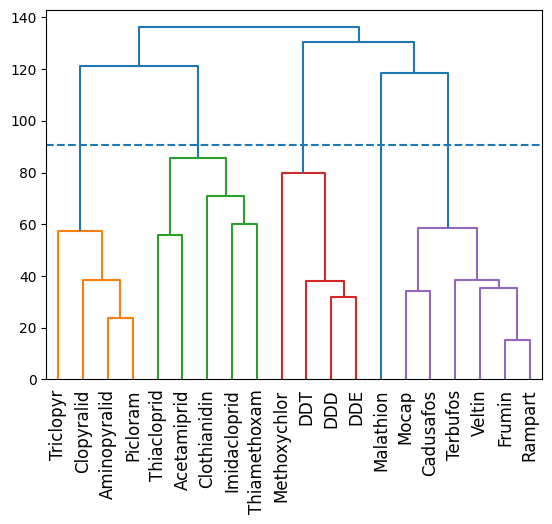
\includegraphics{wp_Manh.png}
        \caption{Dendrogram dla wiązania pojedynczego, metryka odległości Manhattan, dane autoskalowane}
    \end{figure}

    \begin{figure}[H]
        \centering
        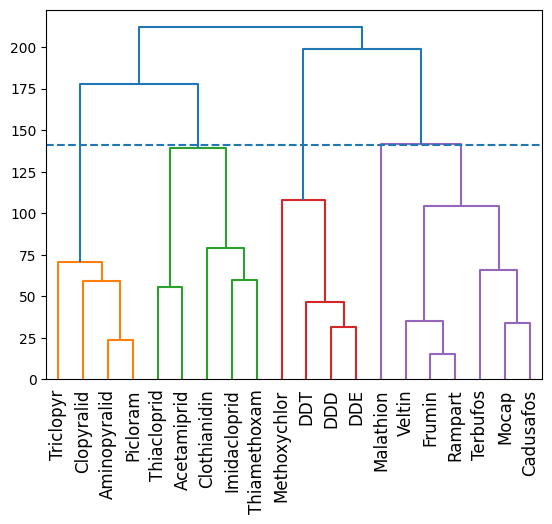
\includegraphics{wc_Manh.png}
        \caption{Dendrogram dla wiązania całkowitego, metryka odległości Manhattan, dane autoskalowane}
    \end{figure}

    \begin{figure}[H]
        \centering
        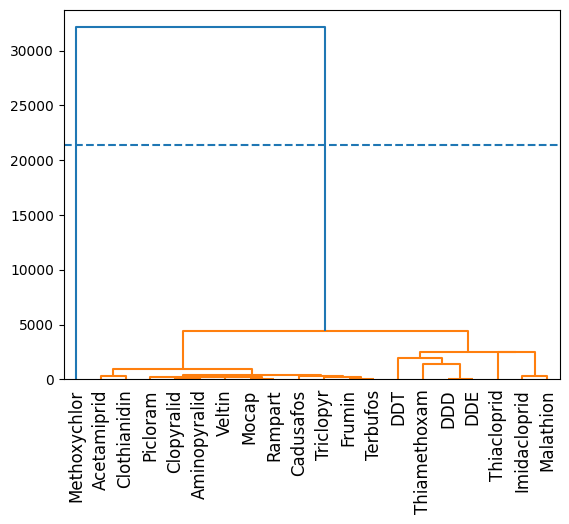
\includegraphics{wp_Euk_b_as.png}
        \caption{Dendrogram dla wiązania pojedynczego, metryka odległości Euklidesowej, dane nieautoskalowane}
    \end{figure}

    \begin{table}[H]
        \centering
        \caption{Porównanie powstałej liczby klastrów oraz najwyższych wartości odległości dla dendrogramów.}
        \begin{tabular}{|c|c|c|}
        \hline
                                                                                                     & \textbf{liczba klastrów} & \textbf{najwyższa wartość odległości} \\ \hline
        \textbf{\begin{tabular}[c]{@{}c@{}}wiązanie pojedyncze\\ odległość Euklidesowa\end{tabular}} & 7                        & 15.55                      \\ \hline
        \textbf{\begin{tabular}[c]{@{}c@{}}wiązanie całkowite\\ odległość Euklidesowa\end{tabular}}  & 6                        & 22.90                      \\ \hline
        \textbf{\begin{tabular}[c]{@{}c@{}}wiązanie pojedyncze\\ odległość Manhattan\end{tabular}}   & 5                        & 136.11                     \\ \hline
        \textbf{\begin{tabular}[c]{@{}c@{}}wiązanie całkowite\\ odległość Manhattan\end{tabular}}    & 5                        & 211.95                     \\ \hline
        \textbf{\begin{tabular}[c]{@{}c@{}}wiązanie całkowite\\ odległość Euklidesowa\end{tabular}}  & 2                        & 32107.06                   \\ \hline
        \end{tabular}
    \end{table}

    Jak widać, powstająca liczba klastrów różni się od siebie w zależności od wybranego typu wiązania oraz metryki odległości.
    Dendrogramy z odległością Manhattan widocznie różnią się pod względem zarówno liczby klastrów oraz najwyższej wartości odległości.
    
    Wartości otrzymane dla danych nieautoskalowanych różnią się znacząco od pozostałych. Powstały wykres jest bardzo skondensowany ze względu na odstającą najwyższą wartość odległości.
    Obserwowany dendrogram możnaby interpretować, że dane dzielą się tylko na 2 zbiory co odbiega od pozostałych wyników.

    Warto zaznaczyć, że dendrogramy poniżej punktu odcięcia, który został ustawiony na $\frac{2}{3}$ wysokości, nieznacznie różnią się od siebie. Co najwyżej pojedynczymi przypadkami.
    Mowa oczywiście o przypadkach dla danych autoskalowanych.

\section{Wnioski i dyskusja}

    Związki: 
    \\\{ Methoxychlor, DDT, DDD, DDE \} - DDT i analogi
    \\\{ Triclopyr, Clopyralid, Aminopyralid, Picloram \} - kwasy pirydynokarboksylowe
    \\\{ Thiacloprid, Acetamiprid, Clothiaridin, Imidacloprid, Thiamethoxam \} - neonikotynoidy
    \\\{ Malathion, Veltin, Frumin, Rampart, Terbufos, Mocap, Cadusafos \} - związki organofosforanowe
    \\w większości przypadków znajdowały się w jednym klastrze, lub ewentualnie, było blisko aby tak się stało na co wskazuje odległość maksymalnie
    jednego wiązania.

    Taką sytuację możnaby interpretować, że dane pochodziły od najprawdopodobniej 4 typów związków. Taka informacja zgadza się z tą otrzymaną od osoby prowadzącej ćwiczenia.
    Po sprawdzeniu substancji potwierdziliśmy, że należą one do podanych wyżej grup pestycydów.

    Jeśli jednak mielibyśmy wskazać, który dendrogram przedstawia informacje najbliższe tych prawdziwych, byłby to ten dla wiązania całkowitego
    i metryki odległości Manhattan dla danych autoskalowanych. Przedstawia on 5 klastrów, jednak wiązanie tworzące ów piąty klaster znajduję się
    tuż na granicy odcięcia.

    Jak widać na powyższym przykładzie HCA, czyli hierarchiczna analiza klastrów, która jest przykładem uczenia maszynowego bez nadzoru dobrze nadaje się
    do podziału zbioru danych na mniejsze, łatwiejsze do interpretacji grupy, jednak potrzebne są do tego odpowiednie narzędzia oraz wiedza do interpretacji wyników.
\end{document}